\documentclass[a4paper,10pt]{scrartcl}
\usepackage[utf8x]{inputenc}
\usepackage{alltt}
\usepackage{upquote}
\usepackage{graphicx}


\begin{document}

\section*{Markov Zooming Map equation -- a detailed example}

This example assumes that you have compiled/installed the code correctly as described in the \texttt{ README} file.
To see if the code is working appropriately, open Matlab and switch to the Markov Zooming Map folder as your working directory. Then execute the following commands:
\begin{alltt}
\% load the provided example graph (a ring of rings) into an adjacency matrix
A = convertPajekToAdjMatrix('ring_of_rings.net');\\
\% assign an output filename
filename = 'test';\\
\% specify a time interval for the analysis
time =logspace(-1,2,100);\\
\% run the actual analysis; note that the time argument is optional, if not
\% provided the time interval is set to the one also used in this example
MarkovZoomingMap(A,filename,time)
\end{alltt}

While the code is running you will see some output for each timepoint provided, which looks similar to this one:
\begin{scriptsize}
\begin{alltt}
...
Attempt 99/100
Iteration 1, moving 100 nodes, looping 1 1 1 times between mergings to code length 4.70389 in 5 modules.
Iteration 2, moving 100 nodes, looping 1 times between mergings to code length 4.70389 in 5 modules.
Attempt 100/100
Iteration 1, moving 100 nodes, looping 1 1 1 times between mergings to code length 4.70389 in 5 modules.
Iteration 2, moving 100 nodes, looping 1 times between mergings to code length 4.70389 in 5 modules.
Done! Code length 4.70389 in 5 modules.
\end{alltt}
\end{scriptsize}


After the code has finished, a folder \texttt{testZoomingMap} should have been created. In this folder you will find two files, a pajek file of the graph and a Matlab file containing the results of the analysis. Load the file and run the script \texttt{script\_plot\_Map\_results}. The resulting figure you obtain should look (apart from the inset) like the one below.
\begin{figure}[tb!]
 \centering
 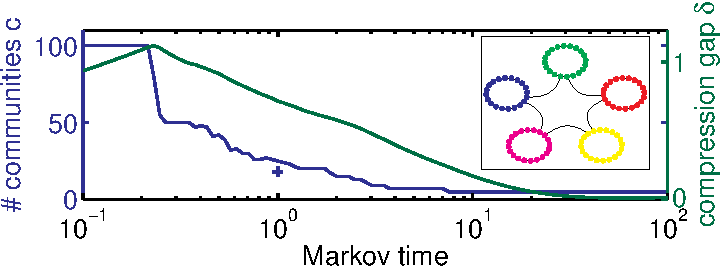
\includegraphics{./test.pdf}
 % test.pdf: 346x128 pixel, 72dpi, 12.21x4.52 cm, bb=0 0 346 128
 \caption{Example analysis ring of rings network. The inset shows the analysed graph.}
 \label{fig:1}
\end{figure}
The dark blue line denotes the number of communities found at a given Markov time, the green line shows the compression gap found (see also reference \cite{Schaub2012} ).
The blue cross denotes the number of communities found by the original Map equation.
The clustering of the nodes is stored in the variables \texttt{clustering} and \texttt{clustering\_new} for the original and the Markov Zooming Map equation respectively.
Likewise the description length and the number of communities found can be found in the variables \texttt{L L\_new N} and \texttt{N\_new}.

\begin{thebibliography}{1}
\bibitem{Schaub2012}
Michael~T. Schaub, Renaud Lambiotte, and Mauricio Barahona.
\newblock ``{E}ncoding dynamics for multiscale community detection: {M}arkov time sweeping for the {M}ap equation.''
\newblock \textit{Physical Reviews E}, 2012, 86(2), 026112; see also arXiv:1109.6642.
\end{thebibliography}

\end{document}
